\chapter{Results}
\label{results}

In this chapter we will present the locomotion gaits obtained with the evolutionary optimization algorithm and we will analyze them for each of the configurations. We will also explain the results obtained after testing the digital hormone-based distributed controller in all the different configurations and its performance compared with our expectations.\\

\section{Evolution results}
\label{results_evolution}

After developing the basic software framework for simulating the locomotion of the modular robot, the locomotion gaits for each of the three configurations were optimized using a Differential Evolution algorithm. The Differential Algorithm main parameters F (the scaling constant) and CR (crossover rate) were left with the ECF default values: 1 and 0.9, respectively.\\

For the rest of the parameters, we used a configuration with a single population of 40 individuals, in order to have a wider search space. The evaluation time of each locomotion gait was configured to 30s, with a simulation resolution of 250\micro s per step, and the oscillator parameters ($A_i$, $O_i$, $\phi_i$, $T$) were restricted to avoid collisions between the different limbs of the modular robot. Table \ref{table:evolution_parameters} shows a summary of the main parameters used for the evolution.\\

\begin{table}[h]
\centering
\begin{tabular}{|c||c|c|} \hline
Parameter & Description & Value \\ \hline \hline
$F$ (Scaling constant) & Amplification of the differential variation & 1 \\ \hline
$CR$ (Crossover rate)  & Probability that a recombination occurs & 0.90 \\ \hline \hline
Population size & Number of individuals on the population &  40 individuals \\ \hline
Evaluation time & Simulation duration  & 30 s \\ \hline
Simulation step & Time of each step of the simulation & 250 \micro s \\ \hline \hline
$A_{max}$ & Maximum amplitude allowed & 80º for \emph{\robotSeven}, 60º for the others \\ \hline
$O_{max}$ & Maximum offset (absolute value) allowed & 45º for \emph{\robotSeven}, 15º for the others \\ \hline
$\phi_{max}$ & Maximum phase allowed & 360º \\ \hline
$f_{max}$ & Maximum frequency allowed & 1.5 Hz \\ \hline
\end{tabular}
\caption{Evolution main parameters}
\label{table:evolution_parameters}
\end{table}

The evolution program was run for appoximately 16h, until stagnation of the best individual fitness value was reached. As evaluating 30s of simulation time results in about 80s / 100s of computing time, depending on the configuration, in those 16h that the program was run a small number of generation were produced (16 for \emph{\robotSeven}, 14 for \emph{\robotNine} and 11 for \emph{\robotEleven}). However, in that number of generations all the configurations had already reached a stagnation point. A plot the fitness value (the robot speed in cm/s) for the different configurations best individual is shown in figure \ref{fig:results_fitness_plot} as a function of the number of generations. The best individual was found at generation 11 for \emph{\robotSeven} and \emph{\robotNine}, and at generation 8 for \emph{\robotEleven}, with values of speed around 9 cm/s.\\

\begin{figure}[h]
		\centering
        \begin{subfigure}[b]{0.31\textwidth}
                \centering
                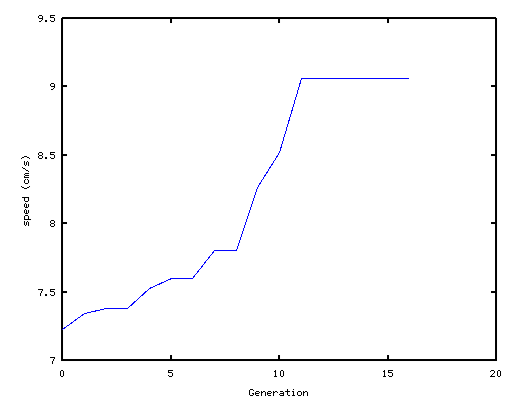
\includegraphics[width=\textwidth]{images/results_7_fitness.png}
                \caption{\robotSeven}
                \label{fig:results_fitness_plot_7}
        \end{subfigure}
        ~
        \begin{subfigure}[b]{0.31\textwidth}
                \centering
                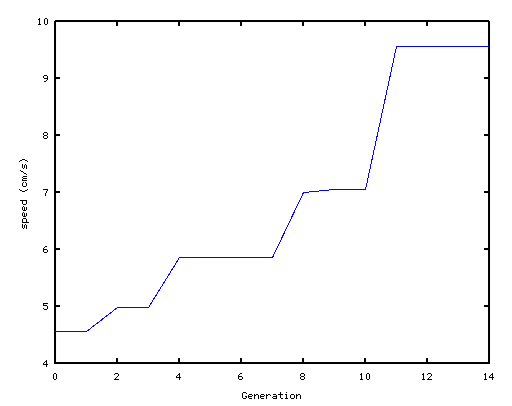
\includegraphics[width=\textwidth]{images/results_9_fitness.png}
                \caption{\robotNine}
                \label{fig:results_fitness_plot_9}
        \end{subfigure}
        ~
        \begin{subfigure}[b]{0.315\textwidth}
         	   \centering
                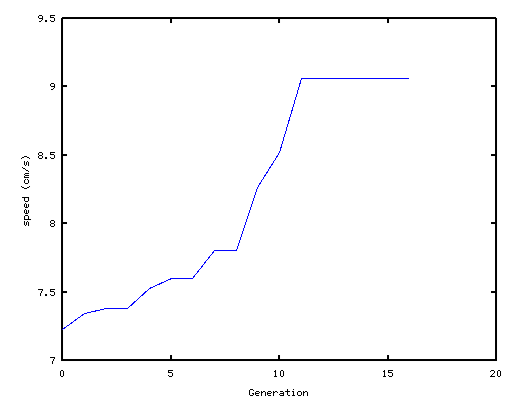
\includegraphics[width=\textwidth]{images/results_7_fitness.png}
                \caption{\robotEleven}
                \label{fig:results_fitness_plot_11}
        \end{subfigure}        
        \caption{Fitness value (robot speed in cm/s) of the best individual as a function of the number of generations}
        \label{fig:results_fitness_plot}
\end{figure}
~\\



\section{Analysis of resulting gaits}
\label{results_gaits}

In this section we will analyze the locomotion gaits generated by the optimized sinusoidal oscillator parameters obtained with the differential evolution optimization, their speed and trajectory and their relationship with those parameters for the three configurations considered in this thesis.\\



%%%%%%%%%%%%%%%%%%%%%% Robot 7 GAITS %%%%%%%%%%%%%%%%%%%%%%%%%%%%%%%%%%%%%%%%%%%%%%%%%%%%%%%%%%%%%%%%%%%%%%%%%
\subsection{\robotSeven}

Table \ref{table:robot_7_parameters} shows the optimal sinusoidal oscillator parameters for the \robotSeven configuration.\\

\begin{table}[H]
\centering
\begin{tabular}{|c||c|c|c|c|c|c|c|} \hline
Parameter & 0 & 1 & 2 & 3 & 4 & 5 & 6 \\ \hline
\hline $A_i$ & 54.06 & 72.14 & 24.76 & 7.21 & 33.67 & 32.00 & 48.96 \\ 
\hline $O_i$ & 34.88 & -31.77 & 36.03 & 30.05 & 39.82 & 24.64 & -38.32 \\ 
\hline $\phi_i$ & 36.34 & 206.12 & 133.29 & 62.80 & 112.13 & 191.15 & 234.73 \\ 
\hline 
\end{tabular}
\caption{\robotSeven ~oscillator parameters}
\label{table:robot_7_parameters}
\end{table}

The resulting gait of this configuration is one in which the robot expands and contracts to displace. The lateral limbs remain almost straight, rolling and using the `leg' modules to advance. The tail modules have an offset towards the limb at the left connector of module 0, and with their movement they contribute to the forward locomotion.\\

\begin{figure}[h]
		\centering
        \begin{subfigure}[b]{0.18\textwidth}
                \centering
                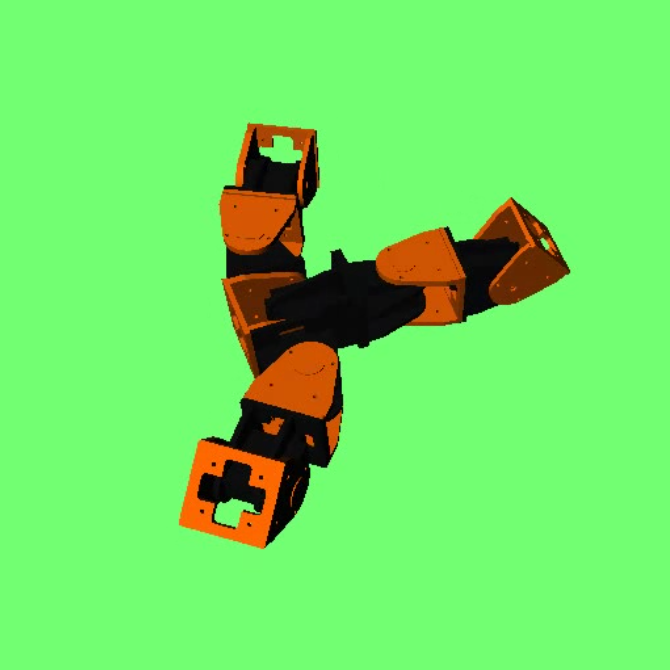
\includegraphics[width=\textwidth]{images/results_7_gait_01.png}
                 \\~
        \end{subfigure}
        ~
        \begin{subfigure}[b]{0.18\textwidth}
                \centering
                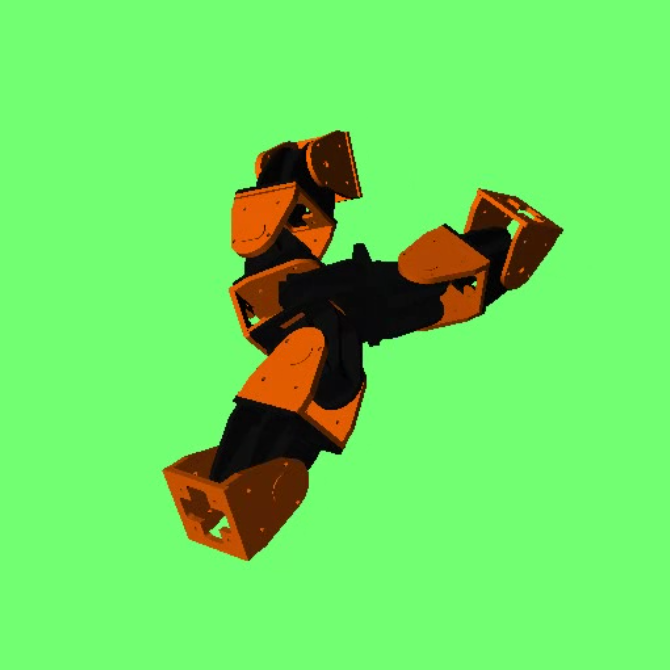
\includegraphics[width=\textwidth]{images/results_7_gait_02.png}
                 \\~
        \end{subfigure}
        ~
        \begin{subfigure}[b]{0.18\textwidth}
         	   \centering
                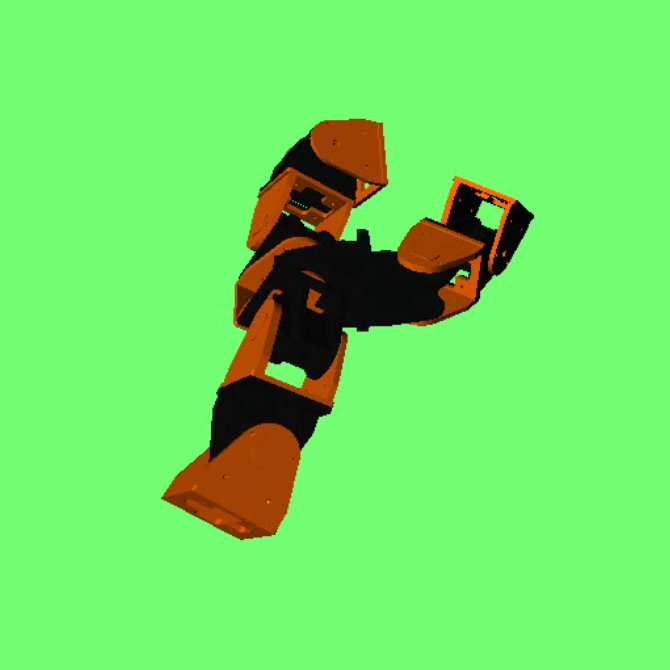
\includegraphics[width=\textwidth]{images/results_7_gait_03.png}
                 \\~
        \end{subfigure}
        ~
        \begin{subfigure}[b]{0.18\textwidth}
         	   \centering
                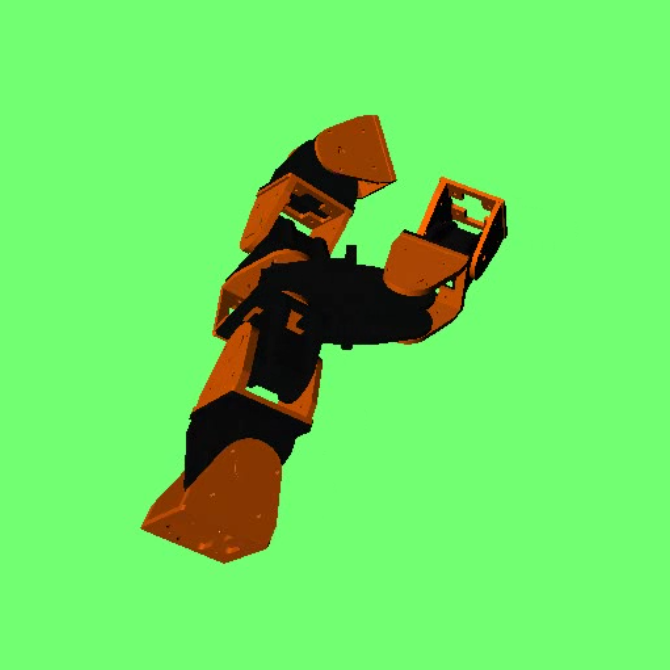
\includegraphics[width=\textwidth]{images/results_7_gait_04.png}
                 \\~
        \end{subfigure}
        ~
        \begin{subfigure}[b]{0.18\textwidth}
         	   \centering
                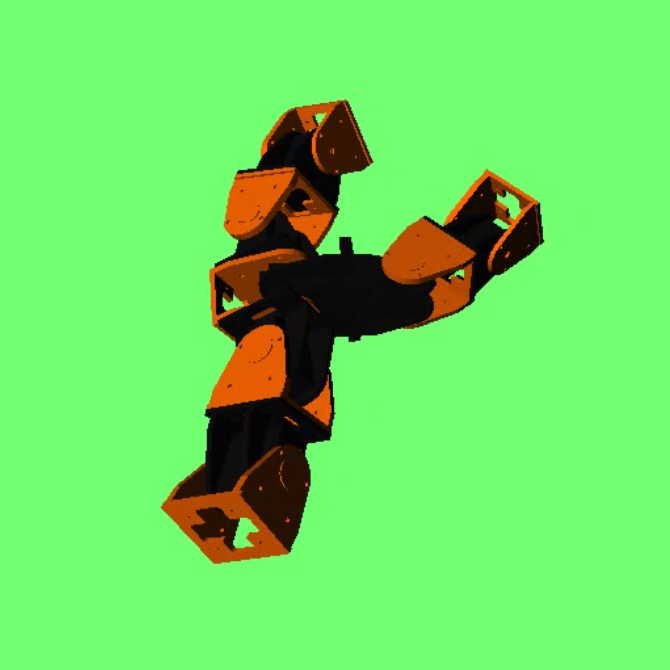
\includegraphics[width=\textwidth]{images/results_7_gait_05.png}
                 \\~
        \end{subfigure}
        ~
                \begin{subfigure}[b]{0.18\textwidth}
                \centering
                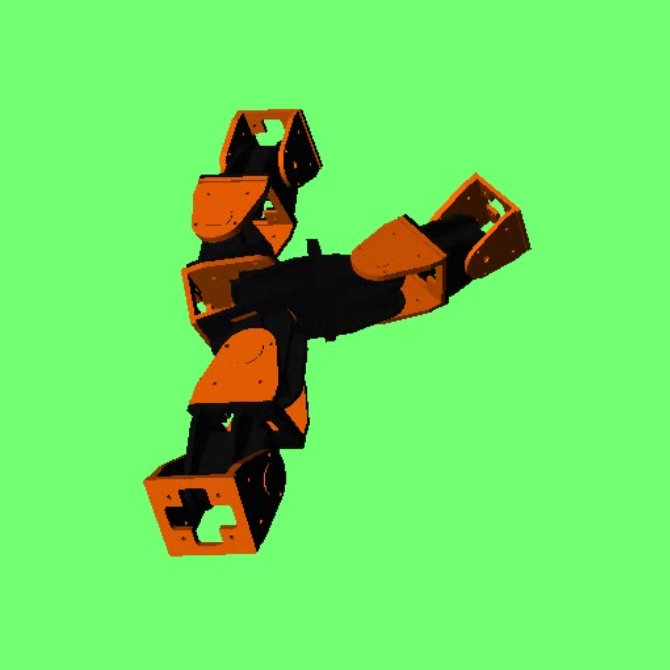
\includegraphics[width=\textwidth]{images/results_7_gait_06.png}
                 \\~
        \end{subfigure}
        ~
        \begin{subfigure}[b]{0.18\textwidth}
                \centering
                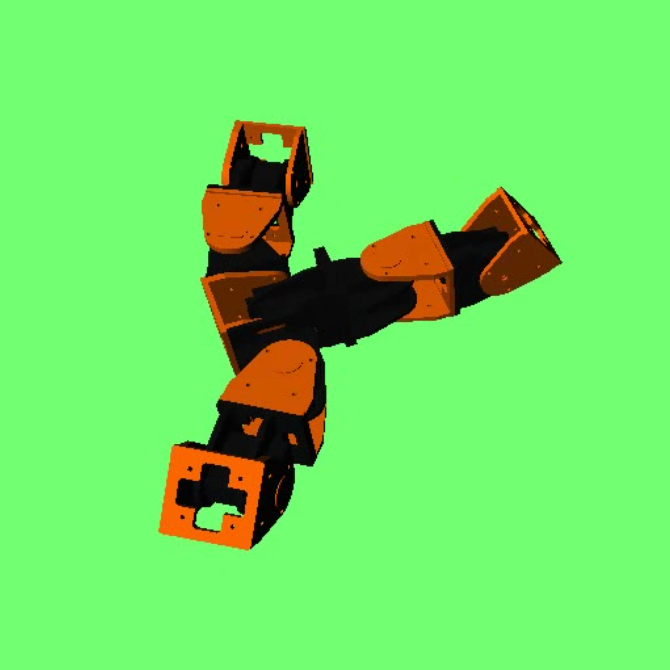
\includegraphics[width=\textwidth]{images/results_7_gait_07.png}
                \\~
        \end{subfigure}
        ~
        \begin{subfigure}[b]{0.18\textwidth}
         	   \centering
                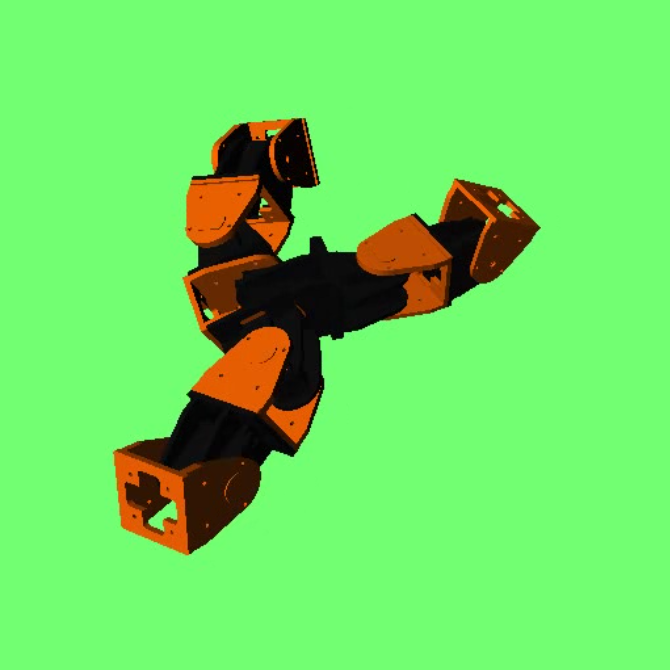
\includegraphics[width=\textwidth]{images/results_7_gait_08.png}
                 \\~
        \end{subfigure}
        ~
        \begin{subfigure}[b]{0.18\textwidth}
         	   \centering
                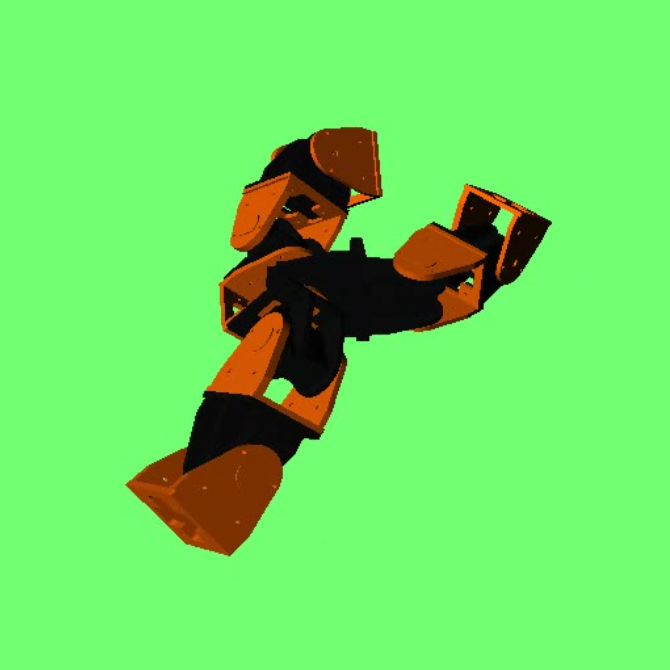
\includegraphics[width=\textwidth]{images/results_7_gait_09.png}
                 \\~
        \end{subfigure}
        \caption{Sequence of the optimal gait obtained for the \robotSeven configuration}
        \label{fig:result_7_gait}
\end{figure}

As we can appreciate, the amplitude and offset values are similar for the two lateral limbs, except for module 3. Since the tail shoulder module (1) has a negative offset, a higher value for the amplitude of module 3 would result in a collision between this limb and the tail, so this low value makes sense.\\

The phase difference between the oscillators is very important for the coordination of the gait. In this case, modules 1, 5 and 6 have a very similar phase, and with their synchronized movement are the modules that contribute the most to the forward movement. Module 0 has a phase difference of approximately 180º with these modules, but as the module is placed upside down, the resulting movement is also in phase with the other modules, favoring the movement of the other modules.\\

The speed of the best individual with this configuration was 9.06 cm/s. Comparing this value with the speed of the best individual in the initial generation, composed by 30 individuals randomly initialized, that is 7.23 cm/s, results in an increase of 125\%.\\

The trajectory followed by this configuration is a straight line directed to the third quadrant, with small oscillations due to the oscillatory nature of the gait, and it is shown in figure \ref{fig:robot_7_trajectory}.\\

\begin{figure}[h]
		\centering
        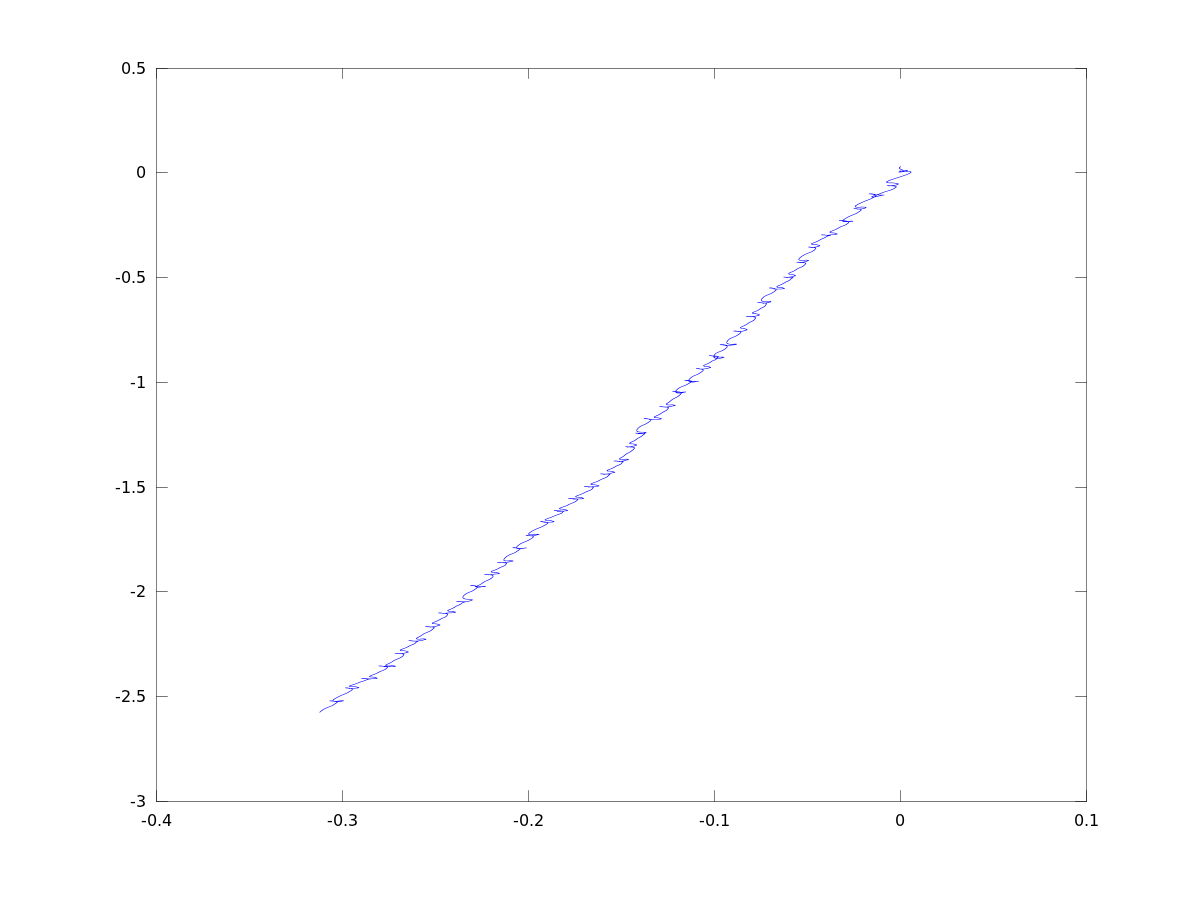
\includegraphics[width=0.6\textwidth]{images/results_7_trajectory.png}
        \caption{Trajectory followed by the \robotSeven configuration}
        \label{fig:robot_7_trajectory}
\end{figure} 

This gait was tested on the physical robot, obtaining the same gait with a similar performance. We tested the gait on different surfaces, and the best results were obtained on the surfaces with a higher friction coefficient, such as carpet and rubber mat. Other surfaces with a low friction coefficient with the robot, such as the floor, made the modular robot slip when performing its gait, resulting in a very small or null advance of the robot.\\ 

\begin{figure}[h]
		\centering
        \begin{subfigure}[b]{0.31\textwidth}
                \centering
                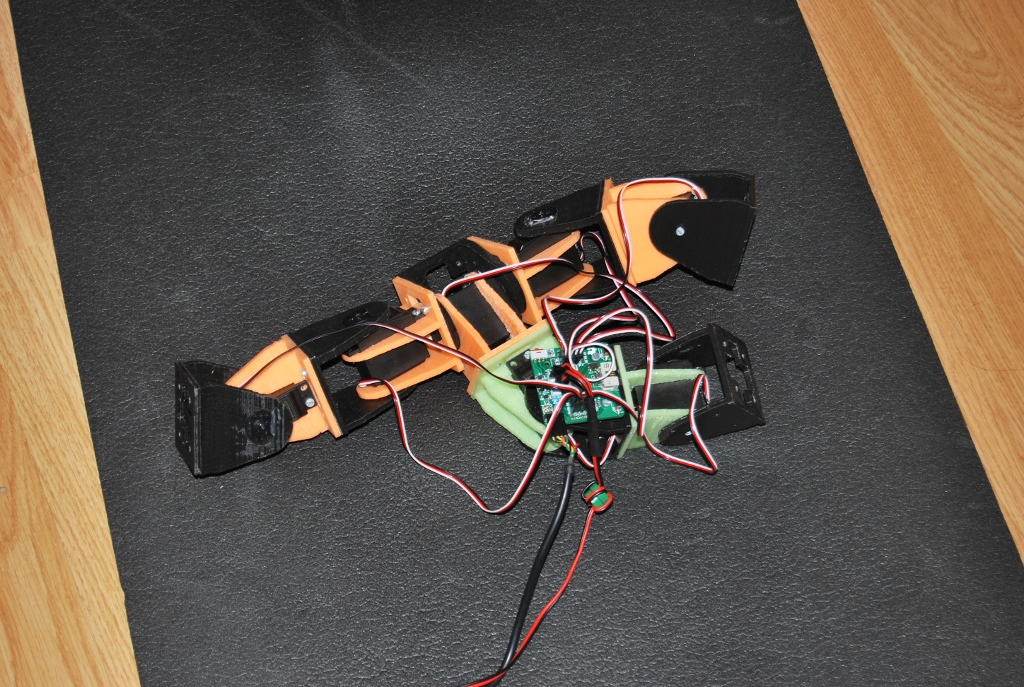
\includegraphics[width=\textwidth]{images/results_7_real_gait_01.jpg}
                 \\~
        \end{subfigure}
        ~
        \begin{subfigure}[b]{0.31\textwidth}
                \centering
                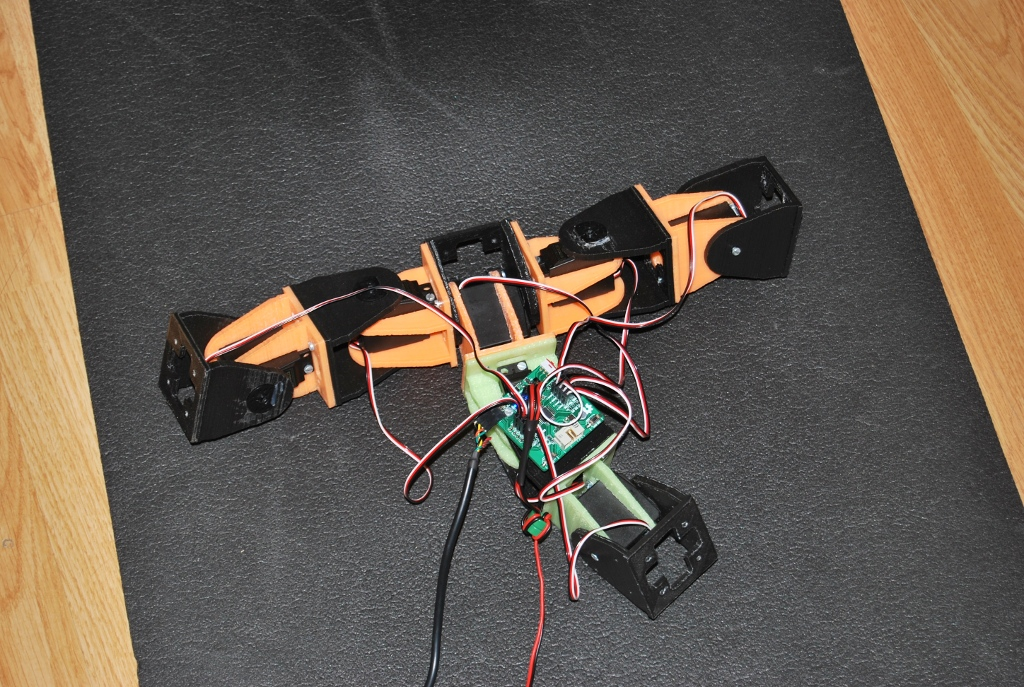
\includegraphics[width=\textwidth]{images/results_7_real_gait_02.jpg}
                 \\~
        \end{subfigure}
        ~
        \begin{subfigure}[b]{0.31\textwidth}
         	   \centering
                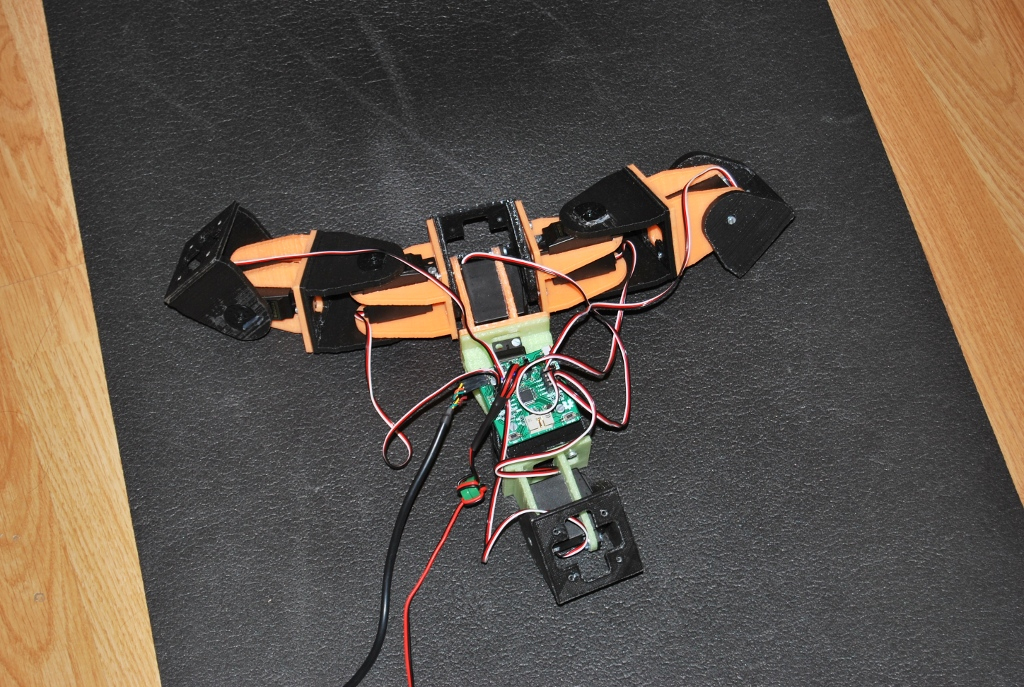
\includegraphics[width=\textwidth]{images/results_7_real_gait_03.jpg}
                 \\~
        \end{subfigure}
        \caption{Testing gait on the modular robot, \robotSeven configuration}
        \label{fig:result_7_real}
\end{figure}


%%%%%%%%%%%%%%%%%%%%%% Robot 9 GAITS %%%%%%%%%%%%%%%%%%%%%%%%%%%%%%%%%%%%%%%%%%%%%%%%%%%%%%%%%%%%%%%%%%%%%%%%%
\subsection{\robotNine}
Table \ref{table:robot_9_parameters} shows the optimal sinusoidal oscillator parameters for the \robotNine configuration.\\

\begin{table}[H]
\centering
\begin{tabular}{|c||c|c|c|c|c|c|c|c|c|} \hline
Parameter & 0 & 1 & 2 & 3 & 4 & 5 & 6 & 7 & 8 \\ \hline
\hline $A_i$ & 37.68 & 32.99 & 54.92 & 37.45 & 4.20 & 19.56 & 56.61 & 38.37 & 13.53 \\ 
\hline $O_i$ & 14.06 & -4.18 & -10.52 & 9.57 & -14.64 & 1.64 & -14.73 & 14.89 & -2.05 \\ 
\hline $\phi_i$ & 76.23 & 26.06 & 255.95 & 37.22 & 123.14 & 110.70 & 1.30 & 155.58 & 109.63 \\ 
\hline 
\end{tabular}
\caption{\robotNine ~oscillator parameters}
\label{table:robot_9_parameters}
\end{table}

This configuration moves in the direction of the limb connected to the back connector of the central module, composed of modules 1 and 4. The limbs connected to the front and back connectors of the central module have a movement that resembles a snake or worm robot, and this movement is helped with the other lateral limbs, which act as arms `rowing' and contributing to the forward movement.\\

\begin{figure}[h]
		\centering
        \begin{subfigure}[b]{0.18\textwidth}
                \centering
                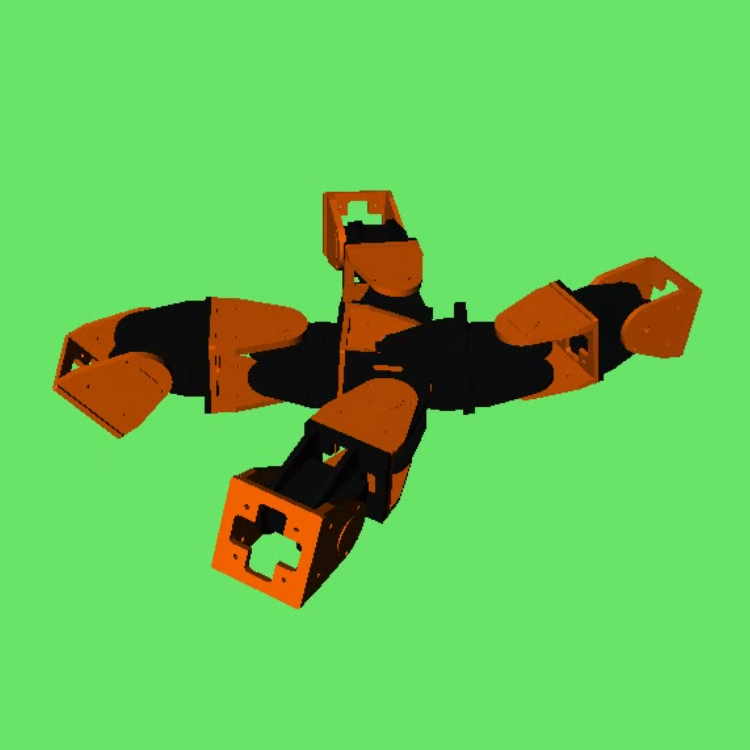
\includegraphics[width=\textwidth]{images/results_9_gait_01.png}
                 \\~
        \end{subfigure}
        ~
        \begin{subfigure}[b]{0.18\textwidth}
                \centering
                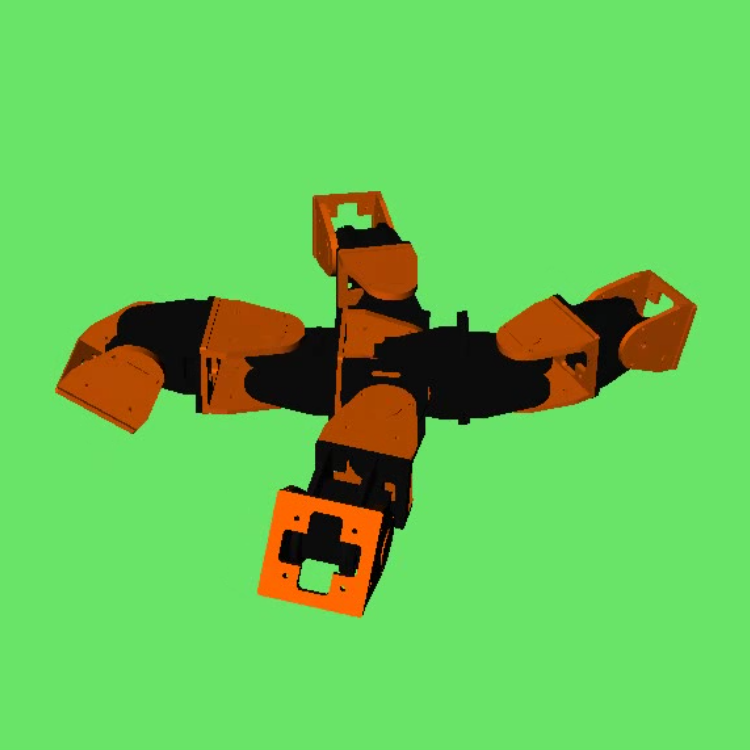
\includegraphics[width=\textwidth]{images/results_9_gait_02.png}
                 \\~
        \end{subfigure}
        ~
        \begin{subfigure}[b]{0.18\textwidth}
         	   \centering
                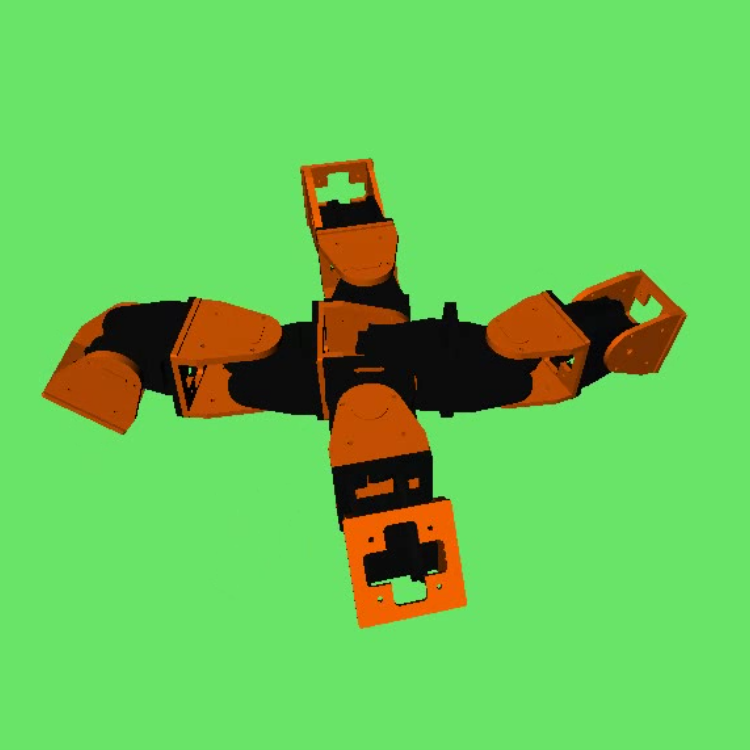
\includegraphics[width=\textwidth]{images/results_9_gait_03.png}
                 \\~
        \end{subfigure}
        ~
        \begin{subfigure}[b]{0.18\textwidth}
         	   \centering
                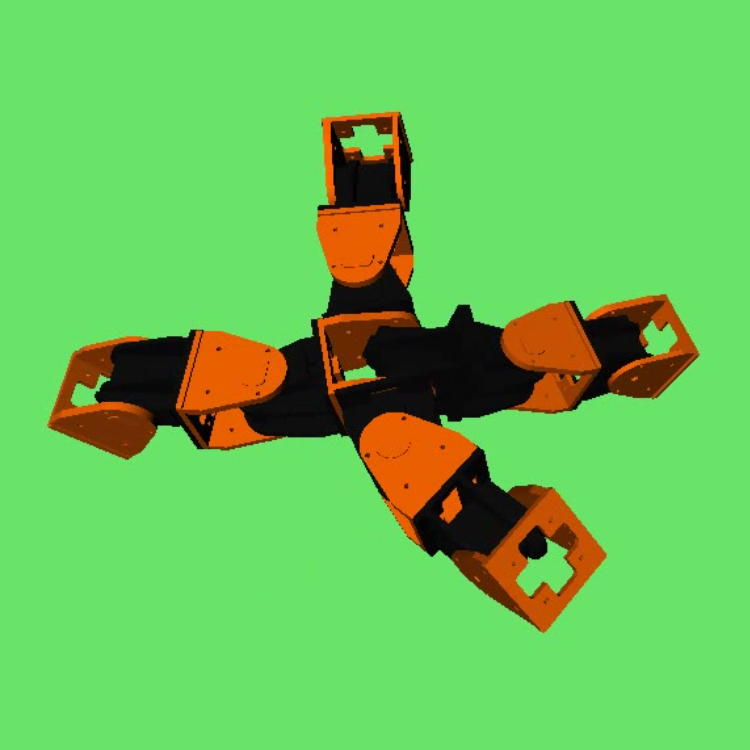
\includegraphics[width=\textwidth]{images/results_9_gait_04.png}
                 \\~
        \end{subfigure}
        ~
        \begin{subfigure}[b]{0.18\textwidth}
         	   \centering
                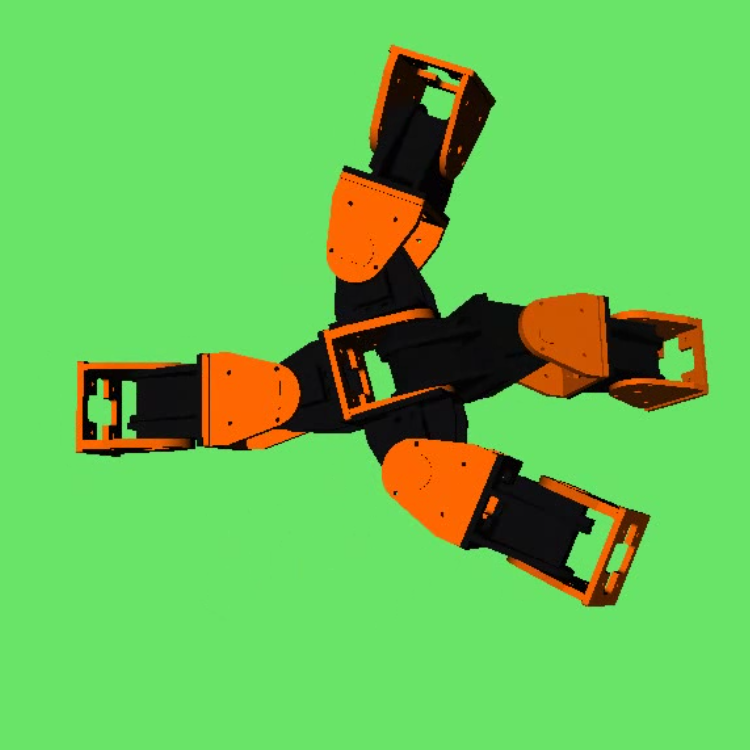
\includegraphics[width=\textwidth]{images/results_9_gait_05.png}
                 \\~
        \end{subfigure}
        ~
                \begin{subfigure}[b]{0.18\textwidth}
                \centering
                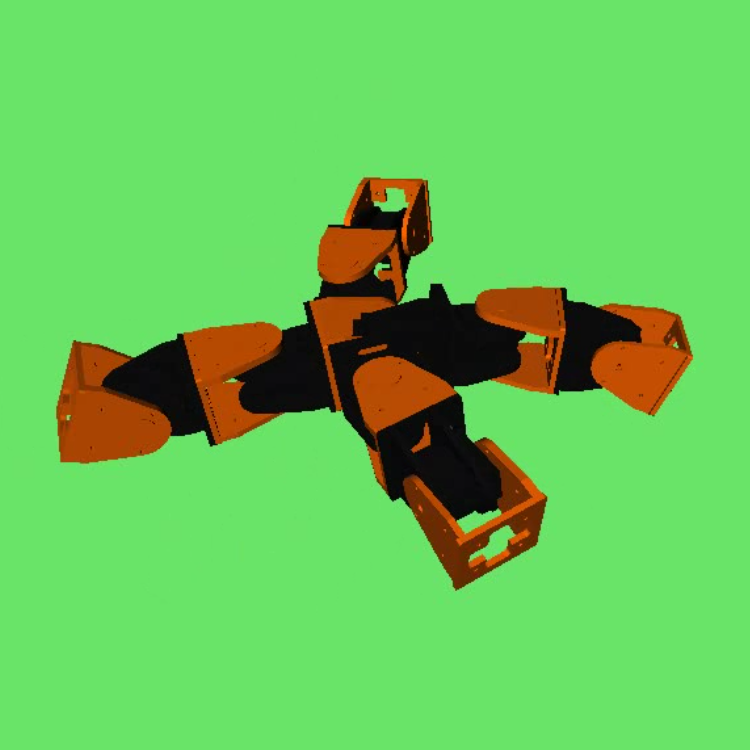
\includegraphics[width=\textwidth]{images/results_9_gait_06.png}
                 \\~
        \end{subfigure}
        ~
        \begin{subfigure}[b]{0.18\textwidth}
                \centering
                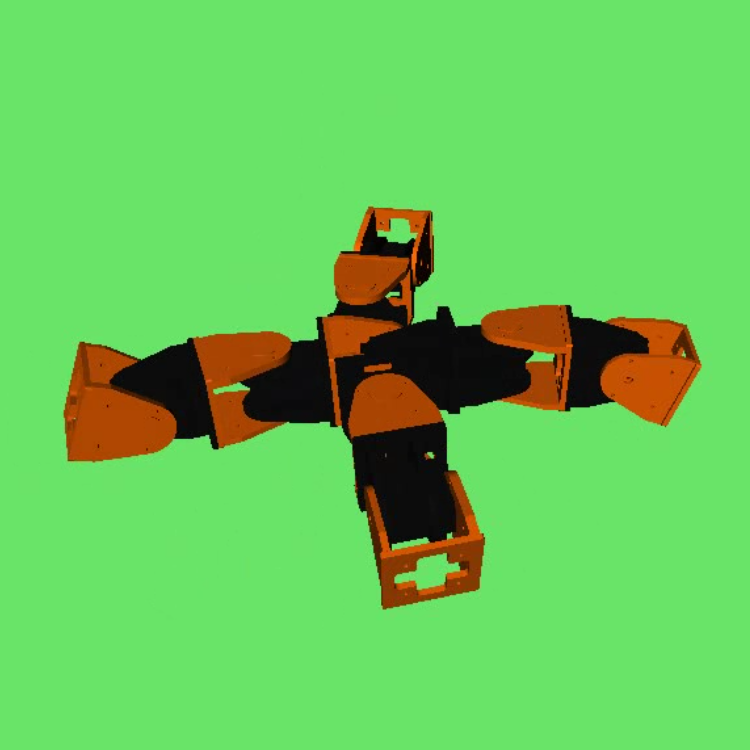
\includegraphics[width=\textwidth]{images/results_9_gait_07.png}
                \\~
        \end{subfigure}
        ~
        \begin{subfigure}[b]{0.18\textwidth}
         	   \centering
                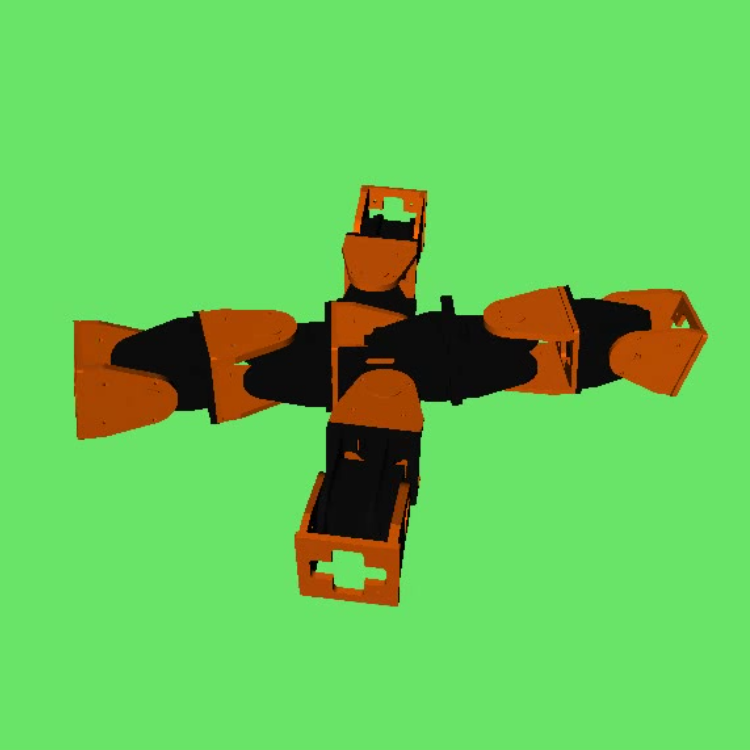
\includegraphics[width=\textwidth]{images/results_9_gait_08.png}
                 \\~
        \end{subfigure}
        ~
        \begin{subfigure}[b]{0.18\textwidth}
         	   \centering
                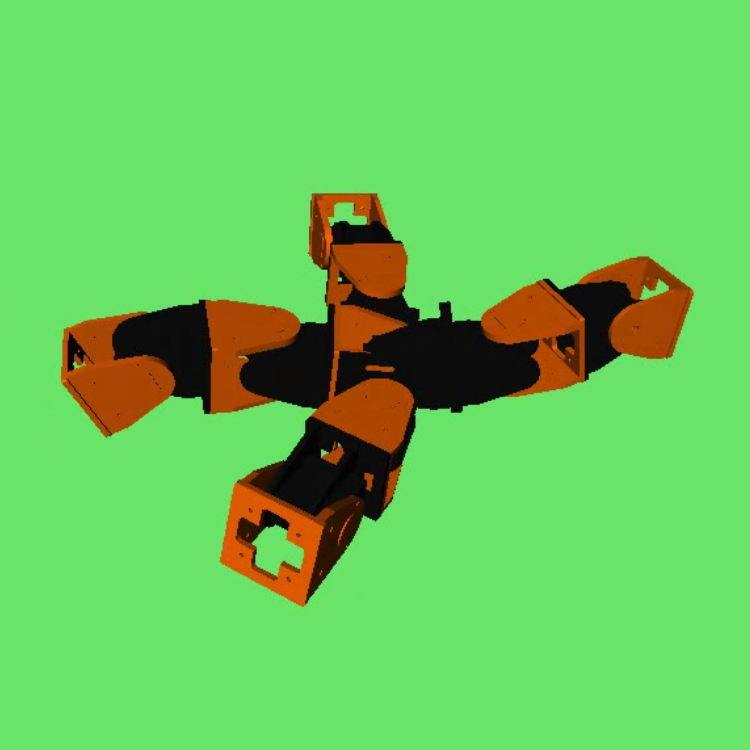
\includegraphics[width=\textwidth]{images/results_9_gait_09.png}
                 \\~
        \end{subfigure}
        \caption{Sequence of the optimal gait obtained for the \robotNine configuration}
        \label{fig:result_9_gait}
\end{figure}

The amplitude and offset values are low due to the constaints imposed to avoid collisions between limbs. Modules 2 and 3, the shoulders of the lateral limbs, have a phase difference of 180º, but as they are placed as mirror images of each other, this results in a movement of these limbs towards the same direction in phase. The other limbs make this `rowing' movement more effective by pushing the robot forward when the lateral limbs are not in contact with the ground.\\

The speed of the best individual with this configuration was 9.57 cm/s. If we compare this value with the speed of the best individual from the 30 individuals randomly initialized of the first generation, 3.32 cm/s, results in an increase of 288\%, almost 3 times better than the random solution.\\

This configuration gait follows a straight line almost parallel to the y axis, with small oscillations due to the oscillatory nature of the gait, which is shown in figure \ref{fig:robot_9_trajectory}.\\

\begin{figure}[H]
		\centering
        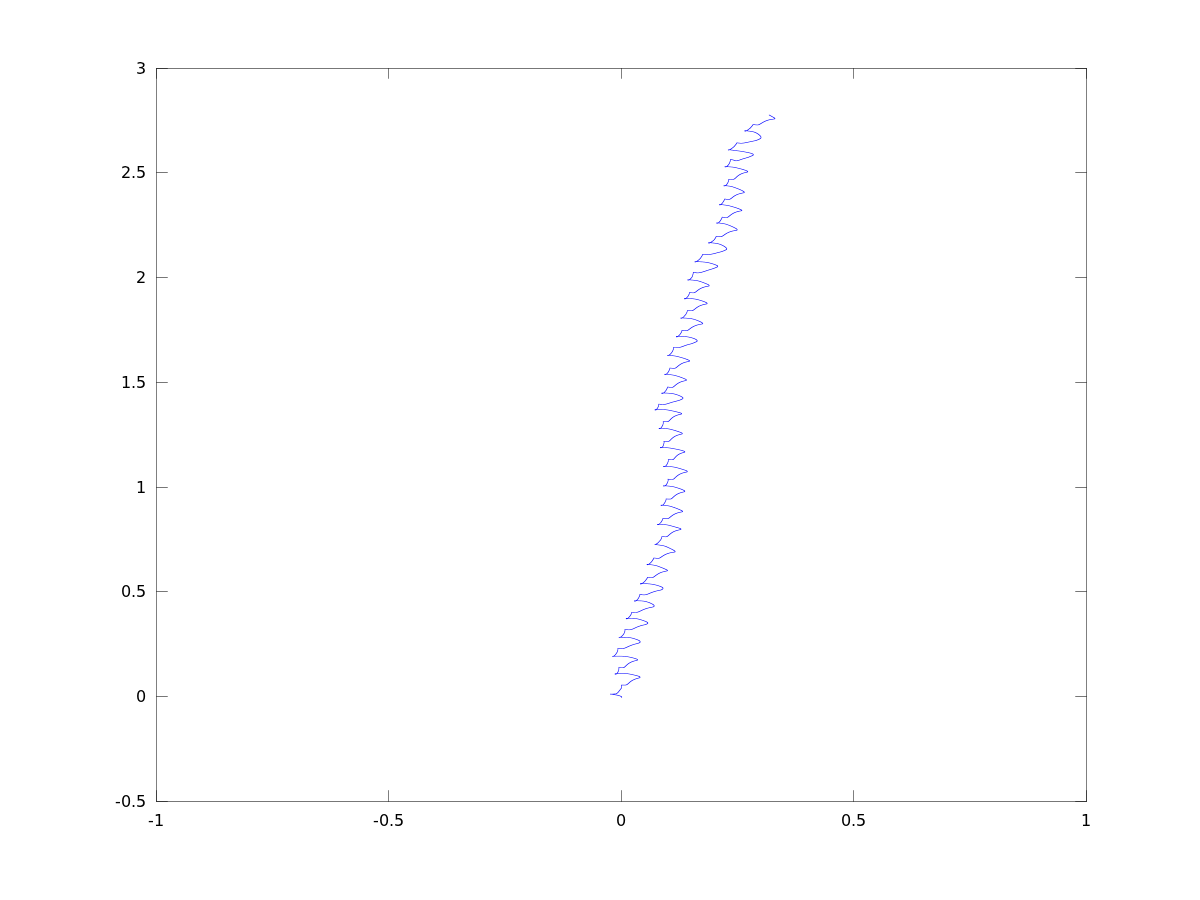
\includegraphics[width=0.6\textwidth]{images/results_9_trajectory.png}
        \caption{Trajectory followed by the \robotNine configuration}
        \label{fig:robot_9_trajectory}
\end{figure} 

Since this configuration is made of 9 modules, and the  modular robot hardware current limit is 8 modules, this gait could not be tested on the real world. Testing this gait requires the use of 2 interconnected control boards, feature that is left as future work. However, the expected results are similar to the previous configuration: a speed close to the values obtained in the simulations, and a better performance over surfaces with a high friction coefficient between them and the robot.\\

\begin{figure}[h]
		\centering
        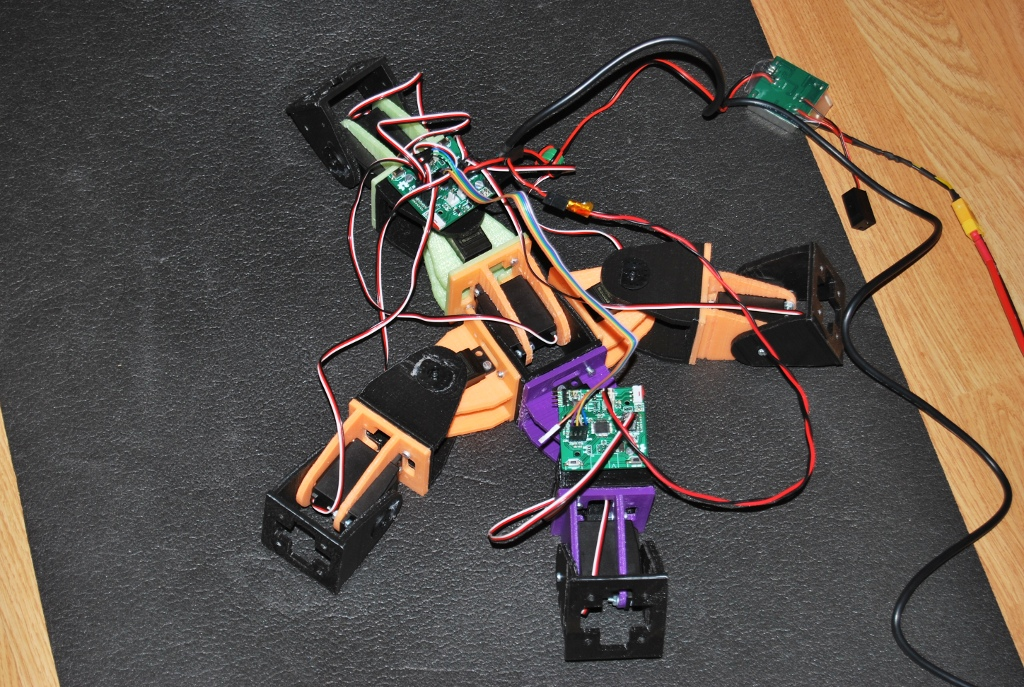
\includegraphics[width=0.45\textwidth]{images/results_9_real_robot.jpg}
        \caption{Modular robot configured as \robotNine}
        \label{fig:robot_9_real}
\end{figure} 

%%%%%%%%%%%%%%%%%%%%%% Robot 11 GAITS %%%%%%%%%%%%%%%%%%%%%%%%%%%%%%%%%%%%%%%%%%%%%%%%%%%%%%%%%%%%%%%%%%%%%%%%%
\subsection{\robotEleven}


Table \ref{table:robot_11_parameters} shows the optimal sinusoidal oscillator parameters for the \robotEleven configuration.\\


\begin{table}[H]
\centering
\begin{tabular}{|c||c|c|c|c|c|c|c|c|c|c|c|} \hline
Parameter & 0 & 1 & 2 & 3 & 4 & 5 & 6 & 7 & 8 & 9 & 10 \\ \hline
\hline $A_i$ & 33.66 & 28.21 & 37.05 & 49.91 & 50.91 & 16.83 & 46.78 & 20.17 & 9.82 & 26.69 & 29.42 \\ 
\hline $O_i$ & 2.91 & 4.19 & 1.63 & -3.04 & -8.53 & -3.82 & -9.07 & -5.51 & -2.93 & 3.14 & -13.14  \\ 
\hline $\phi_i$ & 108.12 & 342.78 & 112.62 & 218.17 & 326.64 & 207.69 & 306.48 & 239.12 & 218.58 & 120.80 & 140.99  \\ 
\hline 
\end{tabular}
\caption{\robotEleven ~oscillator parameters}
\label{table:robot_11_parameters}
\end{table}

This configuration has a gait similar to the typical quadruped gait, with the limbs in the same diagonal moving in phase and in opposite phase as the limbs in the other diagonal to generate a forward movement towards the module 0 direction.\\

\begin{figure}[h]
		\centering
        \begin{subfigure}[b]{0.25\textwidth}
                \centering
                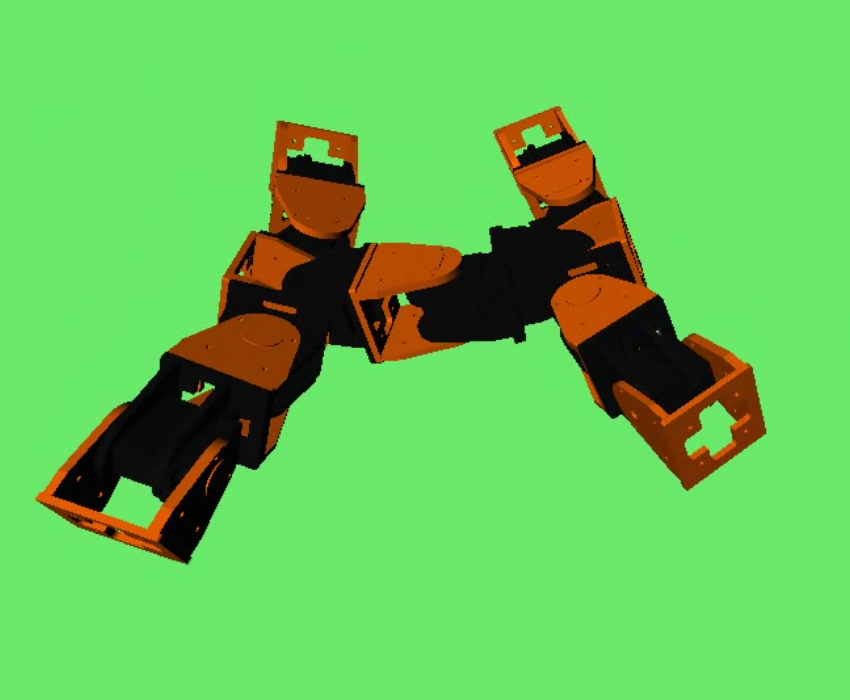
\includegraphics[width=\textwidth]{images/results_11_gait_01.png}
                 \\~
        \end{subfigure}
        ~
        \begin{subfigure}[b]{0.25\textwidth}
                \centering
                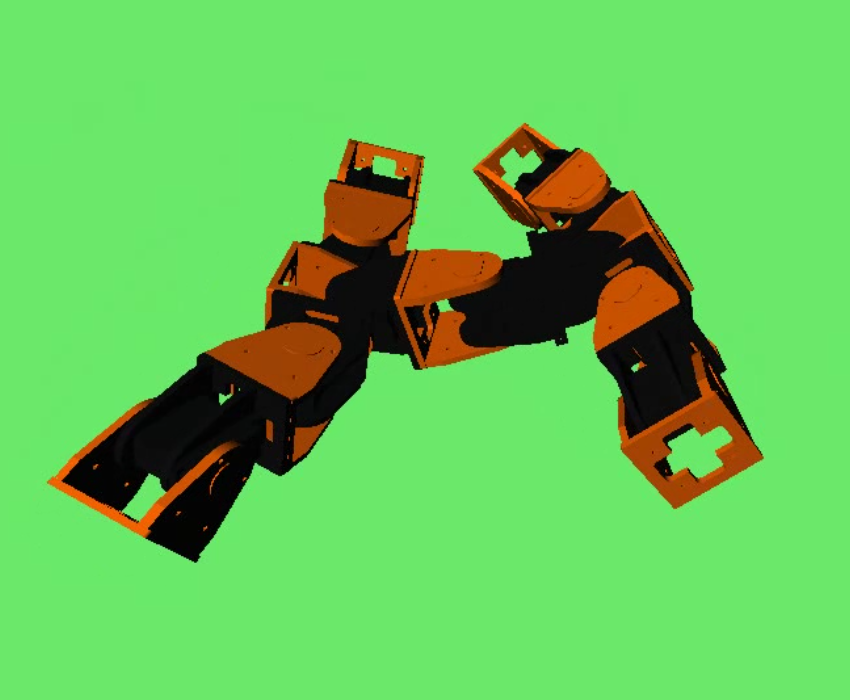
\includegraphics[width=\textwidth]{images/results_11_gait_02.png}
                 \\~
        \end{subfigure}
        ~
        \begin{subfigure}[b]{0.25\textwidth}
         	   \centering
                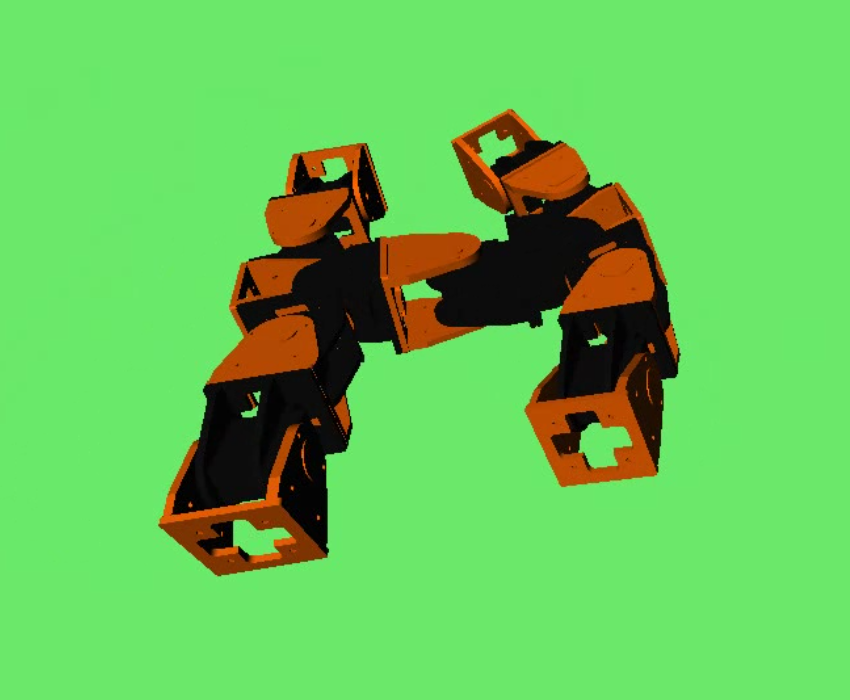
\includegraphics[width=\textwidth]{images/results_11_gait_03.png}
                 \\~
        \end{subfigure}
        ~
        \begin{subfigure}[b]{0.25\textwidth}
         	   \centering
                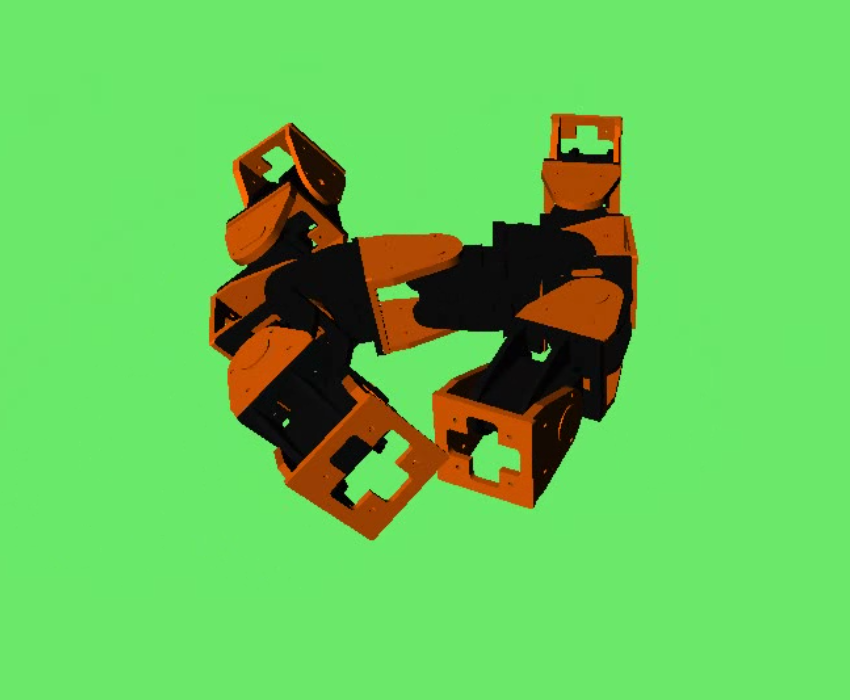
\includegraphics[width=\textwidth]{images/results_11_gait_04.png}
                 \\~
        \end{subfigure}
        ~
        \begin{subfigure}[b]{0.25\textwidth}
         	   \centering
                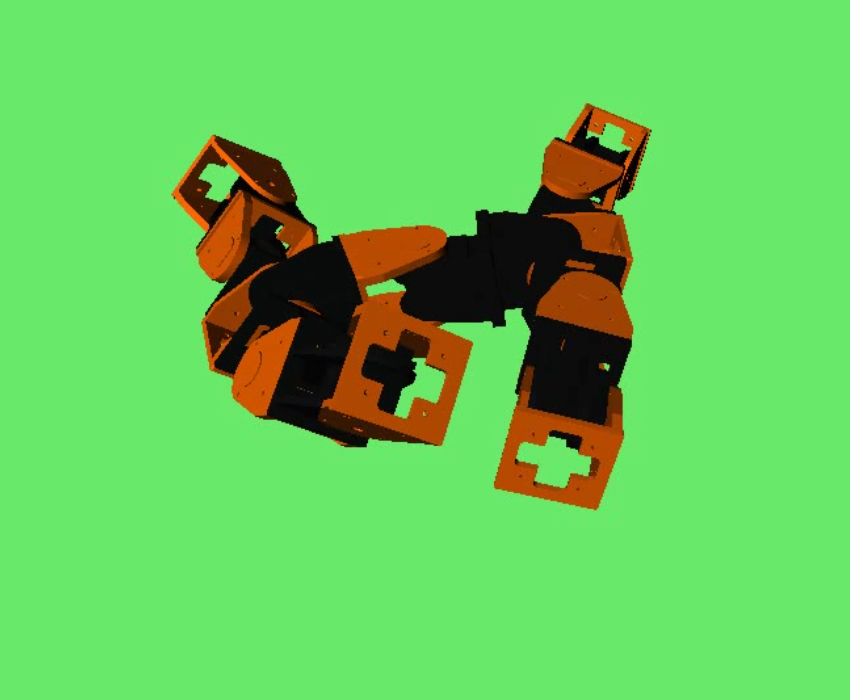
\includegraphics[width=\textwidth]{images/results_11_gait_05.png}
                 \\~
        \end{subfigure}
        ~
                \begin{subfigure}[b]{0.25\textwidth}
                \centering
                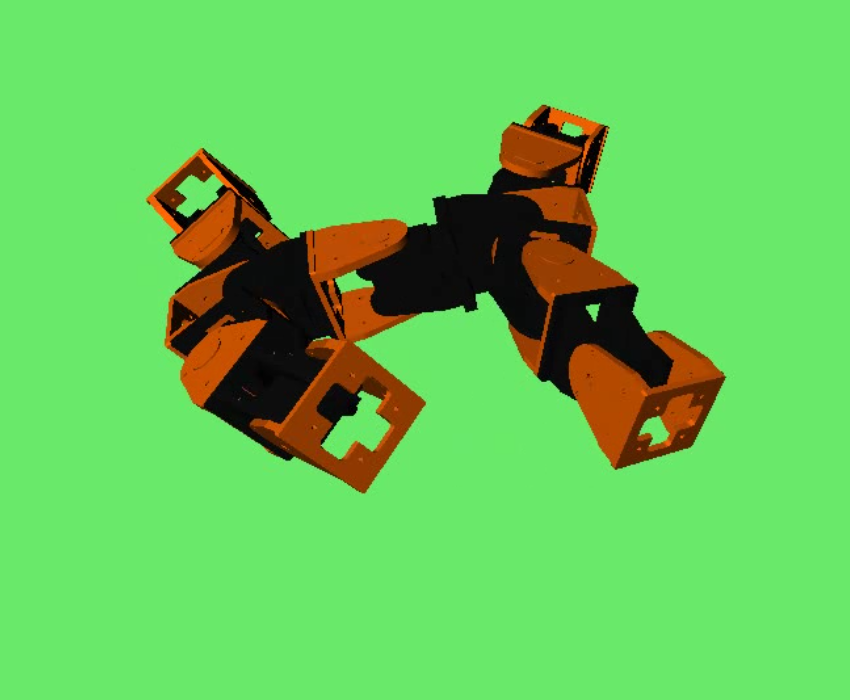
\includegraphics[width=\textwidth]{images/results_11_gait_06.png}
                 \\~
        \end{subfigure}
        ~
        \begin{subfigure}[b]{0.25\textwidth}
                \centering
                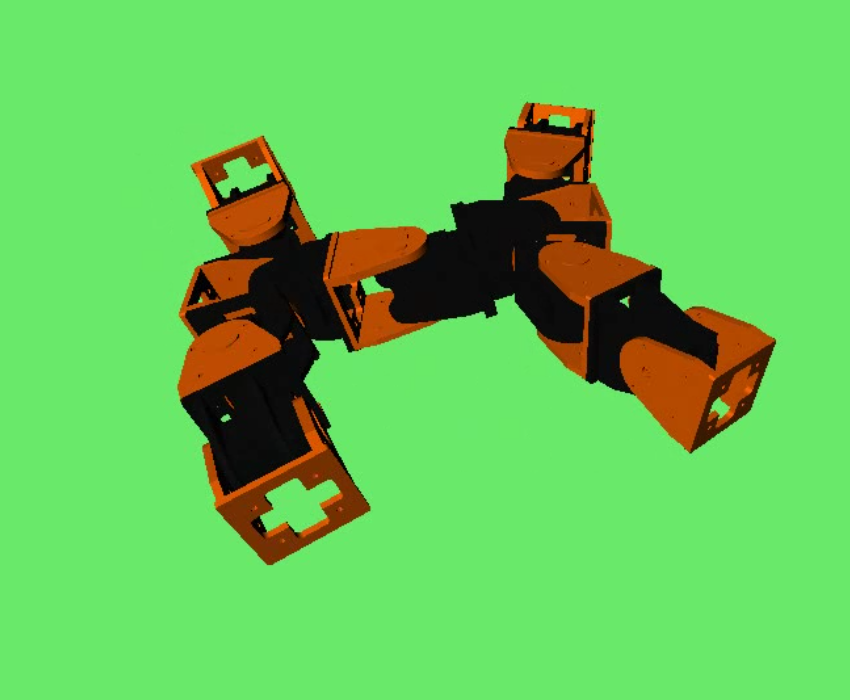
\includegraphics[width=\textwidth]{images/results_11_gait_07.png}
                \\~
        \end{subfigure}
        ~
        \begin{subfigure}[b]{0.25\textwidth}
         	   \centering
                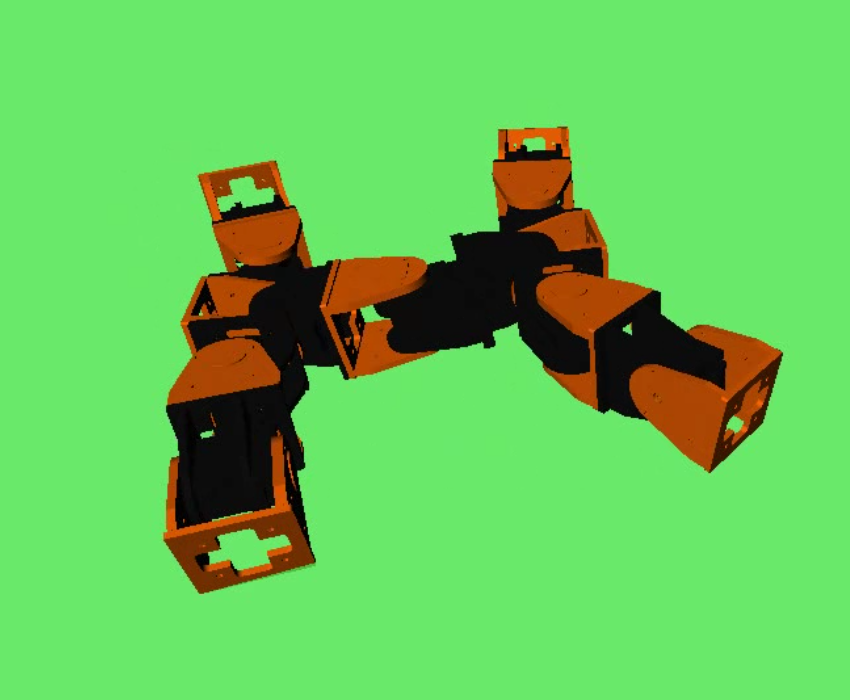
\includegraphics[width=\textwidth]{images/results_11_gait_08.png}
                 \\~
        \end{subfigure}
        ~
        \begin{subfigure}[b]{0.25\textwidth}
         	   \centering
                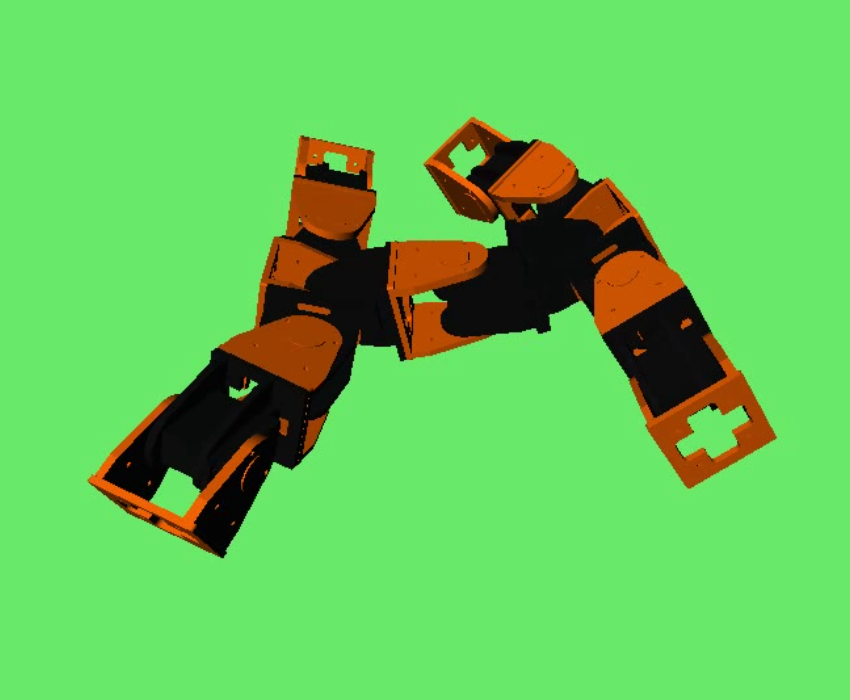
\includegraphics[width=\textwidth]{images/results_11_gait_09.png}
                 \\~
        \end{subfigure}
        \caption{Sequence of the optimal gait obtained for the \robotEleven configuration}
        \label{fig:result_11_gait}
\end{figure}

As with the previous configuration, the amplitude and offset values are low because they were constrained in order to avoid collisions between limbs. Looking at the phase difference between modules 2 and 6, and 3 and 5, we can observe that it is around 180º, but as the modules are mirrored, this results in a movement in phase in the same direction. We can also observe intra-limb coordination, with a phase difference of approximately 120º between the `leg' module and the `shoulder' module of each limb. \\

The best individual with this configuration had a speed of 8.53 cm/s and the best individual among the 30 individuals randomly initialized that compose the initial population was 1.52 cm/s. Comparing them we obtain an increase of 562\%, more than 5 times the speed of the best random individual, which indicates that optimization algorithm generates better gaits than the ones that could be obtained randomly.\\


The trajectory followed by this configuration is also a straight line directed to the third quadrant, with small smooth oscillations due to the oscillatory nature of the gait, and it is shown in figure \ref{fig:robot_11_trajectory}.\\

\begin{figure}[h]
		\centering
        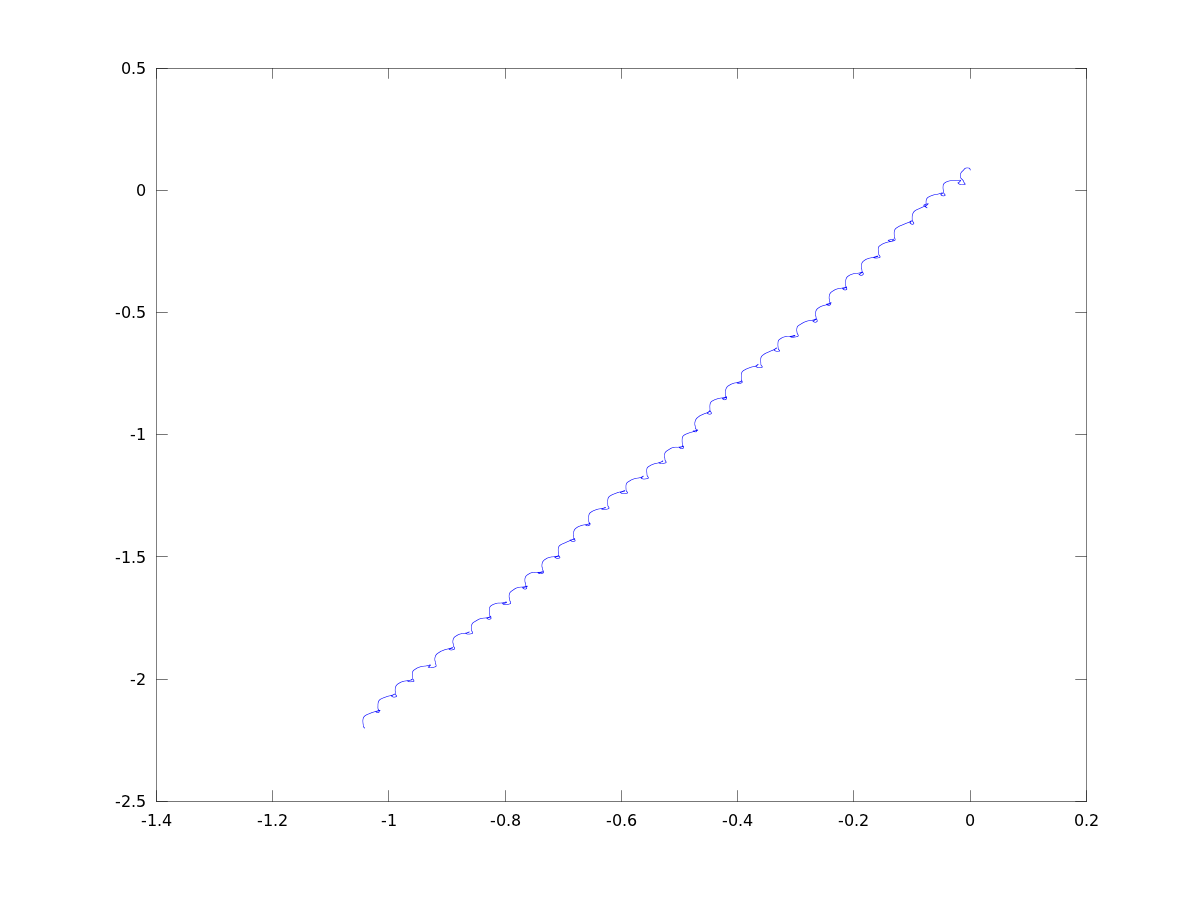
\includegraphics[width=0.6\textwidth]{images/results_11_trajectory.png}
        \caption{Trajectory followed by the \robotEleven configuration}
        \label{fig:robot_11_trajectory}
\end{figure} 

This configuration requires 11 modules and therefore, as the previous configuration, it could not be tested on the real world with the current robotic platform. As with the \robotNine configuration, implementing the communication between the 2 control boards, and testing gaits on this configuration is left as future work.\\

\begin{figure}[H]
		\centering
        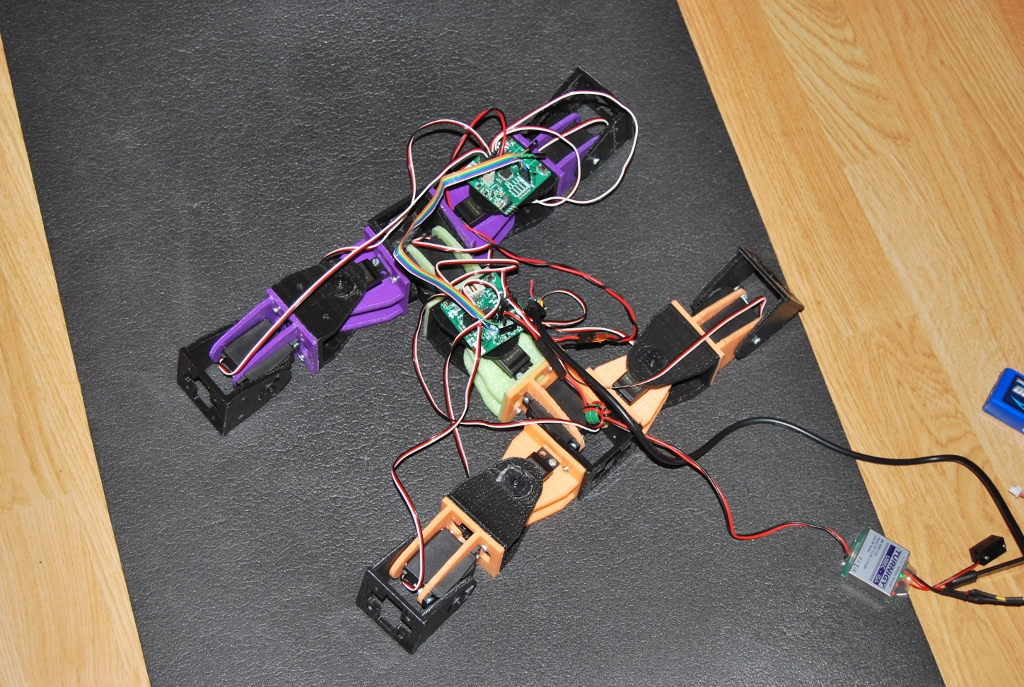
\includegraphics[width=0.5\textwidth]{images/results_11_real_robot.jpg}
        \caption{Trajectory followed by the \robotNine configuration}
        \label{fig:robot_11_real}
\end{figure} 


\newpage
\section{Analysis of hormone-based communication protocol}
\label{results_hormones}

Finally, we will analyze the performance of the hormone-based distributed communication protocol, checking if the controller is able to discover the global configuration of the modular robot as well as the current function of the module inside that configuration. The behavior of the modular robot with this controller will be compared to the behavior of the modular robot with only sinusoidal oscillators with the optimal parameters to check if the speed of the robot decreases when using the hormone-based controller.\\

After running the evolutionary optimization algorithm, the optimal oscillator parameters obtained were extracted and set on the parameter tables, ready to be loaded by the module controller. Once the preparations were finished, the contoller was tested for all the different configurations.\\

Once a brief period of time has passed, in which the robot is finding its current configuration and therefore the resulting gait is chaotic, each module discovers the global configuration of the robot and its role inside that configuration, and sets its oscillator parameters to the corresponding ones according to the values stored in the parameter tables, achieving the optimal locomotion gait for the current configuration.\\

This period of time depends on the communication period being used (i.e. how frequently does the module exchange hormones with the neighboring modules) and the number of communication steps required for a `leg' hormone to travel to the `head' module and for the `head' hormone to travel back to the `leg' module, as explained on section \ref{hormone_algorithm}. This number of steps is different for the three configurations, and it is equal to 6 steps for the \emph{\robotEleven} configuration and 4 steps for the \emph{\robotSeven} and \emph{\robotNine} configurations. The value for the communication period ($T_c$) used for testing the controller was 100 ms, so the initial delay in discovery the configuration and function, and selecting the correct parameters is 400 ms for the \emph{\robotSeven} and \emph{\robotNine} configurations, and 600 ms for the \emph{\robotEleven} configuration.\\

Since the communication period is very large compared to the joint update period (100 ms vs 250 \micro s), this communication does not affect the performance of the robot, which after finding the appropiate gait achieves the same speed as if only the gait is evaluated without controller, by assigning the appropiate parameters to the oscillators by hand.\\ 

Even though reconfiguration is not possible currently, due to limitations in the software framework and in the hardware modules, since the modular robot is able to select gaits correctly for all the three configurations considered with the exact same controller, we can induce that this controller will also work with a reconfiguring modular robot. In that case, the maximum delay for the detection of the new configuration would be the same as the one calculated before for the configurations starting from the initial state, 400 ms for the \emph{\robotSeven} and \emph{\robotNine} configurations, and 600 ms for the \emph{\robotEleven} configuration.